% Solution: Tadelis (2013) Exercise 15.5 "Entry (again)". Input by \solitem.
% Rewritten and deepened from ../pratica-lecture-08-solutions/sol-tadelis-15-5.tex. Check: check_G_L07.py.
\begin{exsol}{Tadelis Exercise 15.5}{316--317}{Exam level}{4}
\asked (a) The extensive form; (b) all pure-strategy BNE, from the matrix; (c) the BNE the incumbent prefers,
and whether it is a PBE; (d) all PBE.

\method Turn the story into terminal payoffs; build the Bayesian game in matrix form (entrant strategies are
type-contingent plans); read off the BNE; then add beliefs at the incumbent's two information sets and ask
for a best reply at each (Tadelis \S15.1--15.2, pp.~304--312). Slides: Lecture~7, frames~27--30 (the
slides' entry game with incomplete information, from Tadelis Ch.~15: a matrix with two BNE, one of which
rests on a threat to fight), 32 (on/off path), 34--36 (Requirements~1--4 and PBE).

\solution
\textbf{Payoffs} (entrant, incumbent). The market is worth $10$, so a share of $s\%$ is worth $s/10$. A weak
entrant pays $6$ to enter at any level.
\begin{center}
\begin{tabular}{llcc}
\toprule
Type & Entry & Accommodate ($A$) & Fight ($F$) \\
\midrule
$T$ & $S$ & $(4,\ 6)$ & $(2,\ 8 - 4) = (2, 4)$ \\
$T$ & $B$ & $(6,\ 4)$ & $(4,\ 6 - 4) = (4, 2)$ \\
$W$ & $S$ & $(4 - 6,\ 6) = (-2, 6)$ & $(0 - 6,\ 10 - 2) = (-6, 8)$ \\
$W$ & $B$ & $(6 - 6,\ 4) = (0, 4)$ & $(0 - 6,\ 10 - 8) = (-6, 2)$ \\
$W$ & $X$ & \multicolumn{2}{c}{$(0,\ 10)$} \\
\bottomrule
\end{tabular}
\end{center}
Fighting a tough entrant raises the incumbent's share by 20 points ($60 \to 80$ after $S$, $40 \to 60$ after $B$)
at a cost of $4$; fighting a weak one takes the whole market at a cost of $2$ (after $S$) or $8$ (after $B$).

\textbf{(a) Tree.} Nature draws $T$ or $W$ with probability $\frac12$ each. $T$ chooses $S$ or $B$; $W$ chooses $S$,
$B$ or $X$ ($X$ ends the game). The incumbent observes the entry size but not the type: one information set
after $S$, one after $B$ (dashed lines).
\begin{center}
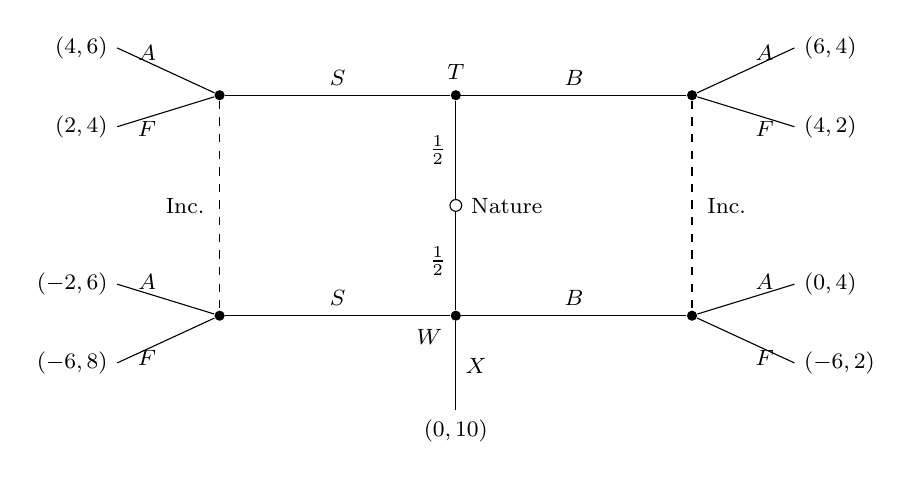
\begin{tikzpicture}[dot/.style={circle,fill,inner sep=1.3pt},every node/.style={font=\footnotesize}]
  \node[circle,draw,inner sep=1.5pt] (n) at (0,0) {};
  \node[right=2pt] at (n) {Nature};
  \node[dot,label=above:{$T$}] (t) at (0,1.4) {};
  \node[dot,label=below left:{$W$}] (w) at (0,-1.4) {};
  \draw (t) -- node[left] {$\frac12$} (n) -- node[left] {$\frac12$} (w);
  \node[dot] (ts) at (-3,1.4) {}; \node[dot] (ws) at (-3,-1.4) {};
  \node[dot] (tb) at (3,1.4) {};  \node[dot] (wb) at (3,-1.4) {};
  \draw (t) -- node[above] {$S$} (ts);  \draw (t) -- node[above] {$B$} (tb);
  \draw (w) -- node[above] {$S$} (ws);  \draw (w) -- node[above] {$B$} (wb);
  \draw (w) -- node[right] {$X$} (0,-2.6) node[below] {$(0,10)$};
  \draw[dashed] (ts) -- (ws); \draw[dashed] (tb) -- (wb);
  \node[left=2pt,align=center] at (-3,0) {Inc.};
  \node[right=2pt,align=center] at (3,0) {Inc.};
  \draw (ts) -- node[above left] {$A$} ++(-1.3,0.6) node[left] {$(4,6)$};
  \draw (ts) -- node[below left] {$F$} ++(-1.3,-0.4) node[left] {$(2,4)$};
  \draw (ws) -- node[above left] {$A$} ++(-1.3,0.4) node[left] {$(-2,6)$};
  \draw (ws) -- node[below left] {$F$} ++(-1.3,-0.6) node[left] {$(-6,8)$};
  \draw (tb) -- node[above right] {$A$} ++(1.3,0.6) node[right] {$(6,4)$};
  \draw (tb) -- node[below right] {$F$} ++(1.3,-0.4) node[right] {$(4,2)$};
  \draw (wb) -- node[above right] {$A$} ++(1.3,0.4) node[right] {$(0,4)$};
  \draw (wb) -- node[below right] {$F$} ++(1.3,-0.6) node[right] {$(-6,2)$};
\end{tikzpicture}
\end{center}

\textbf{(b) Matrix and BNE.} Entrant strategies: (entry of $T$, entry of $W$), six in all. Incumbent strategies:
(reply after $S$, reply after $B$). Each cell averages the two types with weights $\frac12$; for instance
$(SX, AF)$: $T$ enters small and is accommodated $(4, 6)$, $W$ exits $(0, 10)$, so $(2, 8)$. Best replies
underlined:
\begin{center}
\begin{tabular}{r|c|c|c|c|}
\multicolumn{1}{r}{} & \multicolumn{1}{c}{$AA$} & \multicolumn{1}{c}{$AF$} & \multicolumn{1}{c}{$FA$} & \multicolumn{1}{c}{$FF$} \\ \cline{2-5}
$SS$ & $1,\ \br{6}$ & $1,\ \br{6}$ & $-2,\ \br{6}$ & $-2,\ \br{6}$ \\ \cline{2-5}
$SB$ & $2,\ \br{5}$ & $-1,\ 4$ & $1,\ 4$ & $-2,\ 3$ \\ \cline{2-5}
$SX$ & $2,\ \br{8}$ & $\br{2},\ \br{8}$ & $1,\ 7$ & $1,\ 7$ \\ \cline{2-5}
$BS$ & $2,\ 5$ & $1,\ 4$ & $0,\ \br{6}$ & $-1,\ 5$ \\ \cline{2-5}
$BB$ & $\br{3},\ \br{4}$ & $-1,\ 2$ & $\br{3},\ \br{4}$ & $-1,\ 2$ \\ \cline{2-5}
$BX$ & $\br{3},\ \br{7}$ & $\br{2},\ 6$ & $\br{3},\ \br{7}$ & $\br{2},\ 6$ \\ \cline{2-5}
\end{tabular}
\end{center}
Pure BNE (both payoffs underlined): $(SX, AF)$, $(BB, AA)$, $(BB, FA)$, $(BX, AA)$, $(BX, FA)$.

\textbf{(c) The incumbent's favorite.} His payoffs in the five BNE are $8, 4, 4, 7, 7$: he prefers $(SX, AF)$
(tough enters small, weak stays out; accommodate small, fight big). It is \emph{not} a PBE. After $B$ the
incumbent gets $4$ from $A$ and $2$ from $F$ against \emph{either} type, so $A$ is optimal for every belief:
the threat to fight big entry is not credible, and without it the tough type switches to $B$ ($6 > 4$). The
BNE survives only because $B$ is off its path, where a BNE does not test the incumbent's reply.

\textbf{(d) All PBE.} \emph{After $B$:} $A$ for every belief (above). \emph{After $S$:} with
$\mu = \Pr(W \mid S)$, $A$ gives $6$ and $F$ gives $4(1-\mu) + 8\mu = 4 + 4\mu$, so $F$ iff $\mu \ge \frac12$.
\emph{Entrant, given $A$ after $B$:} the tough type gets $6$ from $B$ and at most $4$ from $S$, so he plays $B$;
the weak type gets $0$ from $B$ or $X$ and at most $-2$ from $S$, so he plays $B$ or $X$. Hence no type sends $S$,
$\mu$ is free, and the reply after $S$ may be $A$ (with $\mu \le \frac12$) or $F$ (with $\mu \ge \frac12$):
\begin{center}
\small
\begin{tabular}{llll}
\toprule
Entrant & Incumbent & Beliefs & Inc.\ payoff \\
\midrule
$BB$ (pool on $B$) & $A$ after $B$; $A$ or $F$ after $S$ & $\Pr(W \mid B) = \frac12$; matching $\mu$ & $4$ \\
$BX$ & $A$ after $B$; $A$ or $F$ after $S$ & $\Pr(W \mid B) = 0$; matching $\mu$ & $7$ \\
\bottomrule
\end{tabular}
\end{center}
These are the four BNE other than $(SX, AF)$, now with their beliefs.

\interp Exactly the lesson of the slides' entry game (frames~29--30, 35): the incumbent would like to commit to
fight big entry, but at the moment of choice fighting costs him $2$ whatever the entrant's type, so no belief
can justify it. PBE removes the non-credible plan that a BNE allowed off the path. The surviving equilibria
differ only in whether the weak type, indifferent between big entry and exit, stays out.

\verify \texttt{check\_G\_L07.py} derives the payoff table from the shares and costs, builds the $6\times4$ matrix,
lists the five BNE and the incumbent's payoffs, enumerates the PBE with beliefs on a grid of step $\frac1{60}$
(four profiles; after $S$, $F$ is supported exactly by $\Pr(W \mid S) \ge \frac12$), and checks that $A$ beats $F$
after $B$ for both types. Output: ``Tadelis 15.5: BNE (SX,AF) (BB,AA) (BB,FA) (BX,AA) (BX,FA); incumbent prefers
(SX,AF) = 8, not PBE (A beats F after B); PBE: BB or BX, A after B, F after S iff Pr(W|S) >= 1/2''. Tadelis
prints no answer.

\mistakes
\begin{itemize}
  \item Reading ``increases the market share by 20\%'' as $\times 1.2$. It is 20 percentage points: $60 \to 80$ and
  $40 \to 60$ (and fighting a weak entrant gives $100\%$, as stated).
  \item Forgetting the weak entrant's entry cost $6$ in the entrant's payoffs, or adding it to the incumbent's.
  \item Giving the tough type an $X$ option: his strategy set is $\{S, B\}$, so the matrix has six rows, not nine.
  \item Declaring $(SX, AF)$ a PBE because $B$ is off the path. Off-path beliefs are free, but $F$ after $B$ is
  dominated at both nodes, so no belief supports it.
  \item In (d), stating a single belief after $S$. The off-path belief is free, and both replies after $S$ appear
  in some PBE, each with its own range of $\mu$.
\end{itemize}

\answer{(b) BNE: $(SX, AF)$, $(BB, AA)$, $(BB, FA)$, $(BX, AA)$, $(BX, FA)$. (c) The incumbent prefers $(SX, AF)$
(payoff $8$); it is not a PBE, because after $B$ accommodating beats fighting against both types. (d) PBE: the
tough type enters big, the weak type enters big or exits; the incumbent accommodates after $B$ and, after the
unused small entry, fights iff $\Pr(W \mid S) \ge \frac12$ (accommodates iff $\le \frac12$).}
\end{exsol}
